\textbf{Slagelse kommune}

Slagelse kommune har investeret i Invelox i forbindelse med en lokal produktion af brint i EnergiPark Korsør. Sheerwind producerer ikke selv Invelox, men sælger derimod produktionsrettighederne til andre lokale firmaer. E-Venturi A/S købte i 2014 produktionsrettighederne til Invelox til en værdi af 3,2 millioner kroner. Ud af de 3,2 millioner kroner fik EUE (Energy Universe Europe) aps 600.000 kroner til formidling af projektet, færdiggørelse af kontrakten derudover skulle EUE aps fungere som rådgivere.
E-Venturi manglede fra produktionens start, meget information omkring Invelox-systemet. Dette resulterede i Invelox-systemer, som ikke fungerede. E-Venturi A/S henvendte sig herefter til Sheerwind for at få hjælp til færdiggørelsen af Invelox-systemerne, men dette ville Sheerwind have yderligere betaling for.
Desuden har Slagelse kommune manglet validt data på Invelox, da der ikke en findes en fuld skala model. Derfor nedsatte Slagelse Kommune, i samarbejde med EUE aps, i december 2016 et fagpanel med otte personer, som skulle få adgang til fortrolige data og informationer fra Sheerwind. Disse otte personer har Slagelse kommune og EUE aps ikke ønsket at offentliggøre. Der er dog endnu ingen ny data til rådighed. Hermed står Slagelse kommune indtil videre tilbage med et produkt, som ikke fungerer.

\textbf{Intro til Invelox}

I 2011 fik virksomheden Sheerwind patent på et system kaldet Invelox. Invelox skulle i teorien være bedre og kræve mindre plads end de konventionelle vindmøller. Ifølge Sheerwind larmer de så lidt at de vil være anvendelige i f.eks. byer. Dette vil skabe helt nye muligheder, da dette ikke er muligt hos de konventionelle vindmøller. I 2016 oprettede tre forskellige testcentre. Et i USA, Kina og et i Danmark. 
Sheerwind’s Invelox bygger på en idé om at maksimere energi udbyttet fra vinden ved at hæve vindhastigheden. Deres patenterede design består af fem trin:

\begin{figure}[H]
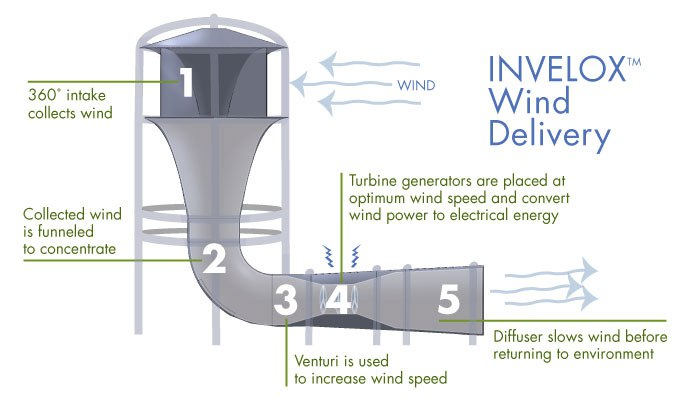
\includegraphics[scale=0.85]{Billeder/invelox_design}
\end{figure}

Første trin er et 360 graders luftindtag med vægge fordelt hele vejen rundt, så det er muligt at opsamle vind fra alle vinkler. Vinden ledes ned til andet trin hvor vinden bliver koncentreret, hermed hæves vindhastigheden. I tredje trin indsnævres røret yderligere og dermed opnås den optimale vindhastigheden. I fjerde trin er turbinerne som omsætter vinden til elektrisk energi ved hjælp af en generator. I femte trin bliver vindhastigheden sænket ved hjælp af en diffuser og bliver herefter ledt ud af Invelox-systemet igen. 
